\chapter{Solution Specification and Design}
\label{ch:solution-design}

This chapter presents the detailed specification and design of the integration methodology. The approach addresses the challenges identified in the state of the art by combining standardized feature extraction through MIOTTA-NPT with a systematic multi-stage pipeline that encompasses label harmonization, data quality assurance, and provenance tracking.

% ══════════════════════════════════════════════════════════════════════════════
\section{Integration Strategy Overview}
\label{sec:strategy}

The integration strategy is structured as a multi-stage pipeline, illustrated in Figure~\ref{fig:pipeline-overview}, that transforms raw network traffic captures from multiple heterogeneous datasets into a single, unified, \gls{ml}-ready dataset. The strategy is guided by the following design principles:

\begin{enumerate}
    \item \textbf{Source-level standardization}: Feature heterogeneity is resolved at the source by reprocessing raw \gls{pcap} captures through a common tool (MIOTTA-NPT), rather than attempting post-hoc feature mapping.

    \item \textbf{Label-level harmonization}: A three-tiered labeling scheme provides classification targets at different granularity levels, enabling both broad and fine-grained intrusion detection experiments.

    \item \textbf{Provenance preservation}: Each record in the unified dataset retains explicit attribution to its source dataset, enabling cross-domain evaluation and analysis of per-source model performance.

    \item \textbf{Quality-first processing}: Data quality assurance is integrated as a core pipeline stage, not an afterthought, ensuring that missing values, outliers, and distribution anomalies are systematically addressed.

    \item \textbf{Extensibility}: The pipeline is designed to accommodate additional datasets (e.g., future custom datasets from the MIoTTA-UPC testbed) without requiring architectural modifications.
\end{enumerate}

\begin{figure}[htbp]
\centering
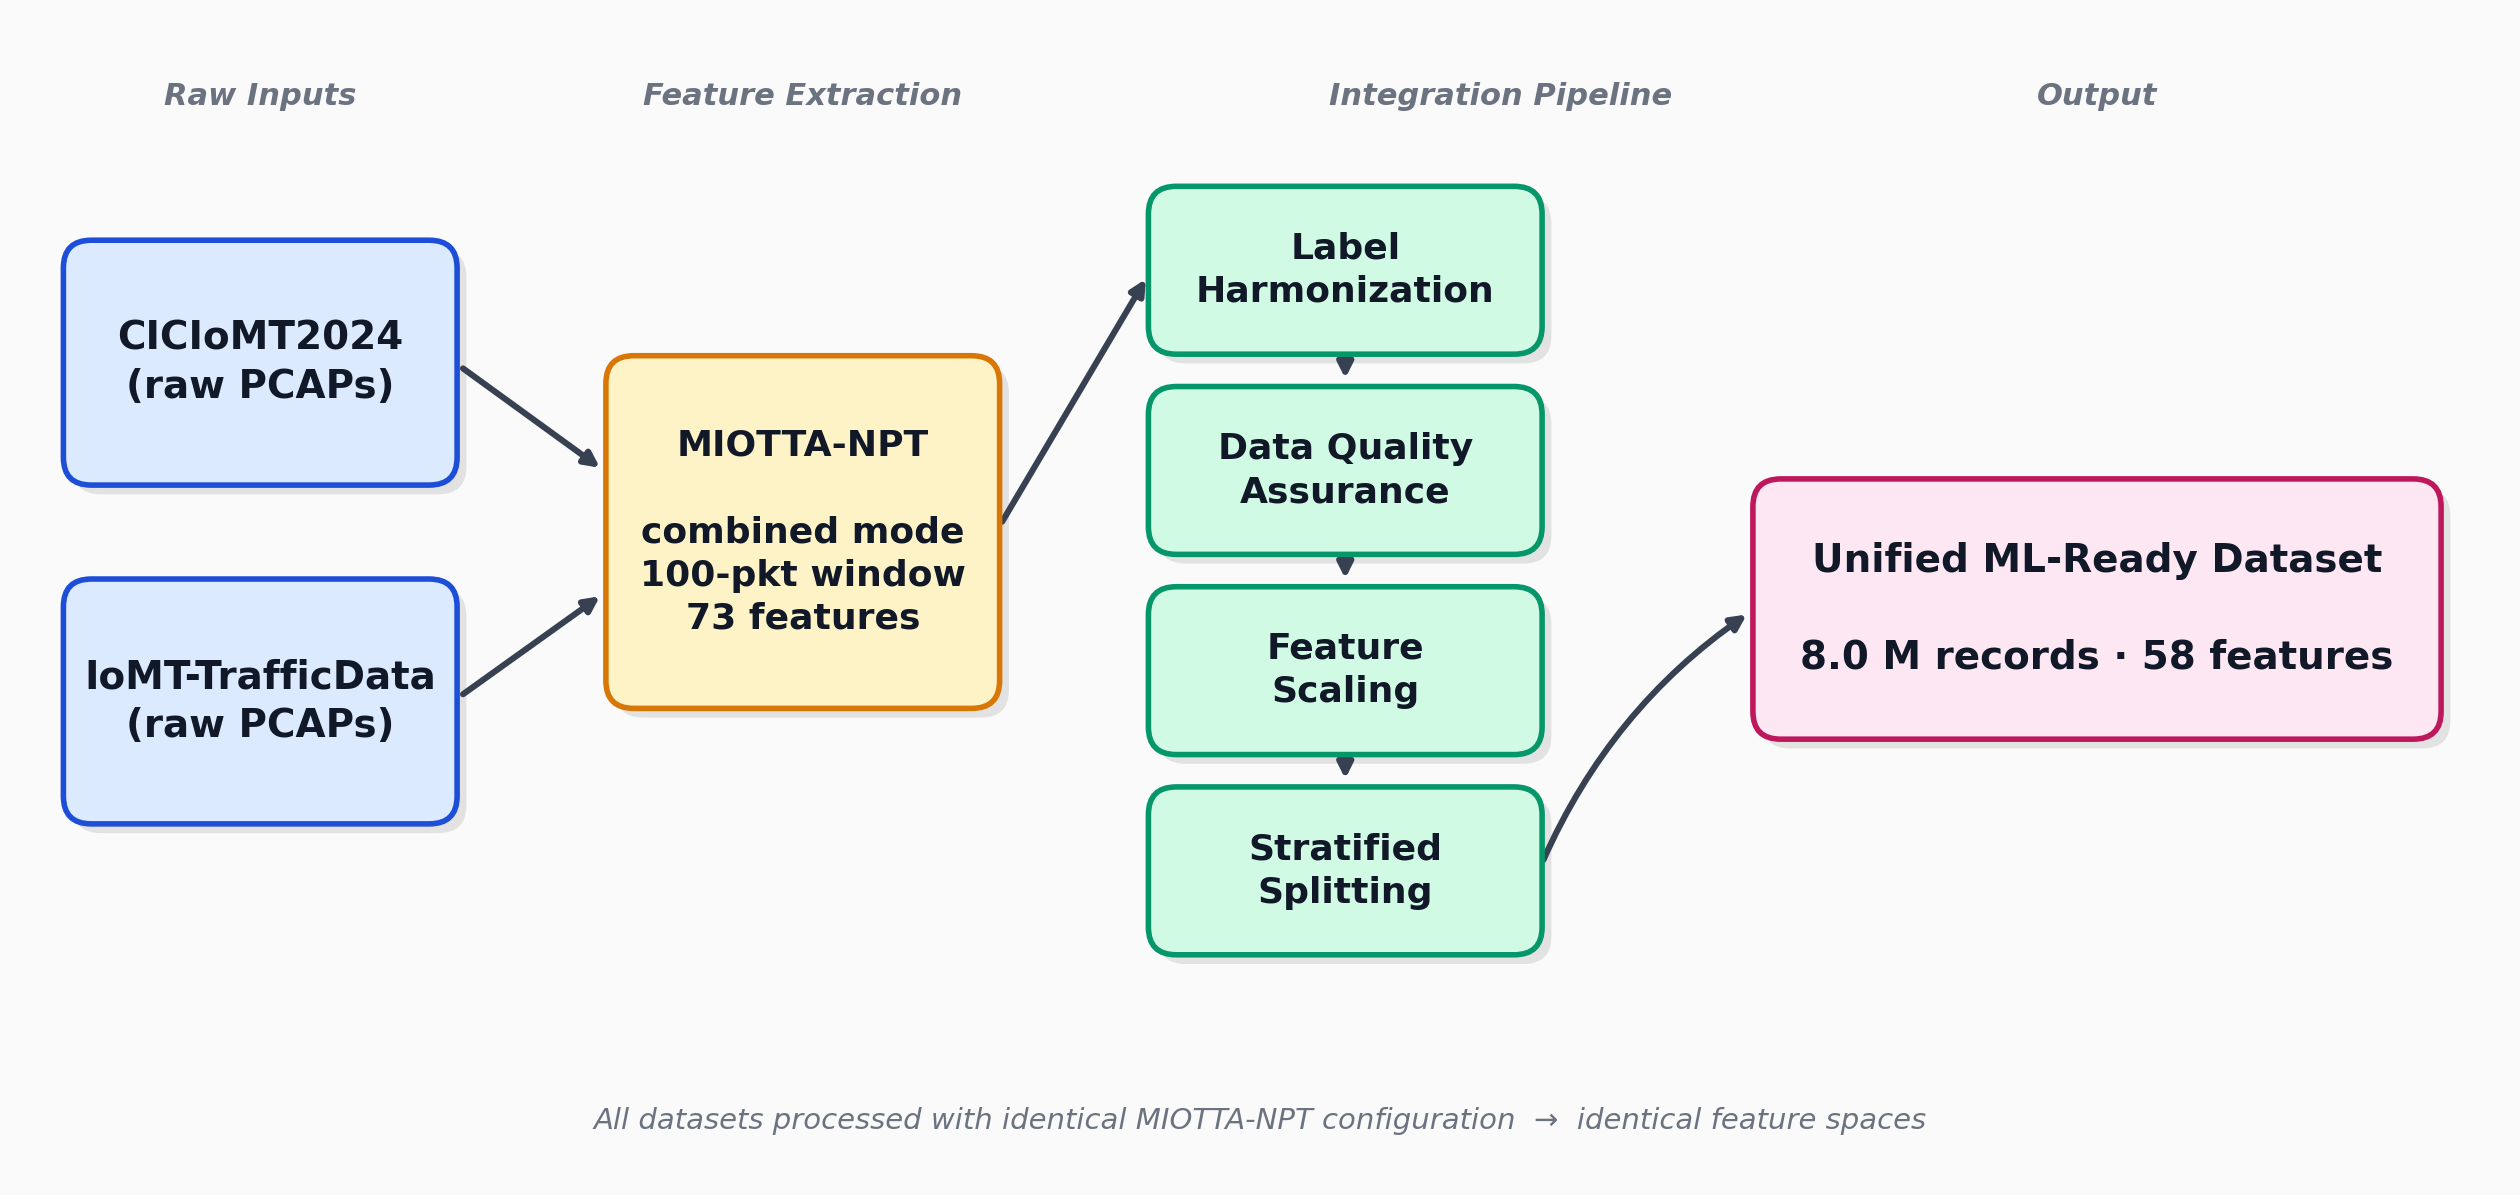
\includegraphics[width=\textwidth]{pipeline_overview.png}
\caption{Overview of the multi-stage integration pipeline. Raw packet captures from CICIoMT2024 and IoMT-TrafficData are processed through MIOTTA-NPT with identical configuration, yielding standardized 73-feature representations. These are then passed through the integration pipeline stages (label harmonization, data quality assurance, feature scaling, and stratified splitting) to produce the final unified ML-ready dataset.}
\label{fig:pipeline-overview}
\end{figure}

% ══════════════════════════════════════════════════════════════════════════════
\section{Dataset Selection and Justification}
\label{sec:dataset-selection}

The selection of datasets for integration is driven by three criteria: (i)~domain relevance to \gls{iomt} security, (ii)~complementarity in attack coverage, and (iii)~availability of raw \gls{pcap} captures for reprocessing. Table~\ref{tab:selection-criteria} summarizes how each dataset meets these criteria.

\begin{table}[htbp]
\centering
\caption{Dataset selection criteria evaluation.}
\label{tab:selection-criteria}
\small
\begin{tabularx}{\textwidth}{@{}l c c X@{}}
\toprule
\textbf{Dataset} & \textbf{Domain} & \textbf{PCAP} & \textbf{Complementary Coverage} \\
\midrule
CICIoMT2024 & IoMT & \checkmark & Multi-protocol IoMT attacks (18 types) \\
IoMT-TrafficData & IoMT & \checkmark & Hospital testbed attacks, data malformation \\
HospNet26 & Real hospital & \checkmark & Real clinical traffic (benign only) — generalization probe \\
\bottomrule
\end{tabularx}
\end{table}

The integration focuses on the two \gls{iomt}-specific datasets:

\begin{itemize}
    \item \textbf{Phase~1 (IoMT integration):} Integrates CICIoMT2024 and IoMT-TrafficData, which share a common \gls{iomt} domain focus, yielding a unified dataset with diverse attack coverage. The resulting artifact is published for community reuse~\cite{unified_iomt_csuc2026}.
\end{itemize}

Additionally, the trained models are evaluated on HospNet26 real hospital network traffic as an out-of-distribution generalization test, without any retraining or adaptation.

% ══════════════════════════════════════════════════════════════════════════════
\section{Feature Standardization via MIOTTA-NPT}
\label{sec:feature-standardization}

\subsection{Processing Configuration}
\label{subsec:processing-config}

All datasets are processed through MIOTTA-NPT using an identical configuration to ensure strict feature space alignment:

\begin{itemize}
    \item \textbf{Mode}: Combined (flow + window), which provides the richest feature representation by capturing both per-flow statistics and window-level temporal aggregations.
    \item \textbf{Window size}: 100 packets, providing a balance between temporal context and computational tractability.
    \item \textbf{Feature set}: The full set of combined-mode features, yielding 73 features per record (the subset of the 103 total features that applies to the combined mode).
\end{itemize}

The choice of the combined mode is motivated by several factors: (i)~it captures both flow-level semantics (who is communicating, how much data is exchanged) and window-level temporal patterns (traffic behavior over a fixed packet window), (ii)~it provides a sufficiently rich feature space for diverse \gls{ml} architectures, and (iii)~the resulting feature count (73) is manageable for both traditional and deep learning models.

\subsection{Resulting Feature Space}
\label{subsec:feature-space}

After processing through MIOTTA-NPT, each dataset produces records with an identical set of 73 features. These features can be organized into the following functional groups:

\begin{enumerate}
    \item \textbf{Connection metadata} (5 features): Flow identifier, window number, protocol type, IP-related fields.
    \item \textbf{Packet size statistics} (6 features): Minimum, maximum, mean, and standard deviation of packet lengths; total bytes; total packet size.
    \item \textbf{Directional metrics} (14 features): Forward/backward packet counts, byte totals, payload sizes, header sizes, and per-second rates.
    \item \textbf{Flow dynamics} (6 features): Rate, source/destination rates, magnitude, radius, covariance, variance ratio.
    \item \textbf{TCP flag distributions} (12 features): Counts and ratios of SYN, ACK, FIN, RST, PSH, ECE, CWR, and URG flags.
    \item \textbf{Temporal features} (6 features): Forward/backward/flow inter-arrival times, timestamps.
    \item \textbf{Protocol indicators} (14 features): Binary or count indicators for HTTP, HTTPS, DNS, TCP, UDP, ARP, ICMP, SSH, SMTP, IRC, DHCP, Telnet, LLC, IGMP, IPv4.
    \item \textbf{Window-level aggregations} (10 features): Header length, TTL, inter-arrival time at window level, initial RTT, connection state indicators.
\end{enumerate}

The strict identity of the feature spaces across datasets---verified empirically as described in Chapter~\ref{ch:execution}---eliminates the need for any feature mapping or alignment procedures.

\subsection{Progressive Deployment of MIOTTA-NPT}
\label{subsec:progressive-miotta}

The pipeline is designed to be agnostic to the number of input datasets: adding a new MIOTTA-processed dataset requires only the creation of a corresponding label mapping (Section~\ref{sec:label-harmonization}) and its inclusion in the concatenation stage. This extensibility also accommodates future datasets generated from the MIoTTA-UPC testbed under development at the university.

% ══════════════════════════════════════════════════════════════════════════════
\section{Integration Architecture}
\label{sec:two-phase}

\subsection{Phase 1: IoMT Semantic Integration}
\label{subsec:phase1}

Phase~1 focuses on the integration of the two \gls{iomt}-specific datasets (CICIoMT2024 and IoMT-TrafficData), both of which have been processed through MIOTTA-NPT with identical configuration. Since the MIOTTA-NPT processing guarantees structural compatibility at the feature level, the integration effort in this phase concentrates on:

\begin{enumerate}
    \item \textbf{Cross-dataset feature verification}: Confirming that the MIOTTA-processed datasets share identical column names, data types, and value ranges.
    \item \textbf{Label harmonization}: Mapping the different attack labels from each dataset into a unified three-level labeling scheme (Section~\ref{sec:label-harmonization}).
    \item \textbf{Data quality normalization}: Applying consistent missing value treatment, infinity value handling, and zero-variance feature removal across both datasets.
    \item \textbf{Source attribution}: Adding a provenance column to track the origin of each record.
\end{enumerate}

The \textit{semantic} nature of this phase refers to the careful attention paid to ensuring that the mapped labels carry consistent meaning across the integrated dataset, and that any dataset-specific characteristics (e.g., NaN values in TCP flag features for non-TCP traffic) are understood and handled consistently.

% ══════════════════════════════════════════════════════════════════════════════
\section{Label Harmonization}
\label{sec:label-harmonization}

The absence of a common labeling convention across datasets necessitates a systematic harmonization procedure. This thesis defines a three-level labeling hierarchy, each level serving a distinct analytical purpose:

\subsection{Three-Level Labeling Scheme}
\label{subsec:label-levels}

\begin{description}
    \item[Level 1 --- Binary (\texttt{label\_binary}):] Classifies each record as either \texttt{Benign} or \texttt{Attack}. This level is useful for basic intrusion detection (is there an attack?) and provides the most balanced class distribution.

    \item[Level 2 --- Category (\texttt{label\_category}):] Groups attack types into six operational categories used in this thesis: \texttt{Benign}, \texttt{DDoS}, \texttt{DoS}, \texttt{MQTT}, \texttt{Reconnaissance}, and \texttt{Spoofing}. The operational mapping adopts a dedicated \texttt{MQTT} category: all MQTT-related attacks (\texttt{MQTT-DDoS-*}, \texttt{MQTT-DoS-*}, \texttt{MQTT-Malformed\_Data}, and \texttt{MQTT Malaria}) are grouped under \texttt{MQTT}. The remaining categories retain nature-based semantics. This level supports multi-class classification at a practical operational level, enabling security analysts to understand both attack nature and protocol-oriented behavior.

    \item[Level 3 --- Fine-grained (\texttt{label\_fine}):] Preserves the original attack type labels from each dataset (e.g., \texttt{DDoS\_TCP\_Flood}, \texttt{ARP\_Spoofing}), with normalization applied to ensure consistent formatting. This level enables the most detailed analysis but may exhibit significant class imbalance due to the uneven representation of specific attack types across datasets.
\end{description}

\subsection{Mapping Strategy}
\label{subsec:label-mapping}

For each dataset, an explicit mapping dictionary defines the correspondence between the original labels and the three harmonized levels. These mappings are developed based on:

\begin{itemize}
    \item The attack type descriptions provided in the original dataset publications~\cite{dadkhah2024ciciomt, areia2024iomt}.
    \item Analysis of the attack execution methodologies described by the dataset authors.
    \item Consultation with the thesis advisors to resolve ambiguous cases where an attack type could plausibly belong to multiple categories.
\end{itemize}

The mapping dictionaries are maintained as configuration artifacts within the integration pipeline, enabling transparent auditing and modification as needed.

% ══════════════════════════════════════════════════════════════════════════════
\section{Data Quality Assurance}
\label{sec:quality}

Data quality issues, if unaddressed, can introduce noise, bias, or artifacts into the unified dataset. The pipeline incorporates the following quality assurance procedures:

\begin{enumerate}
    \item \textbf{Missing value treatment}: Features with NaN values (e.g., TCP flag statistics for windows containing only non-TCP traffic) are imputed with 0 when the NaN arises from the absence of the relevant protocol, or flagged for removal if the missingness rate exceeds a configurable threshold.

    \item \textbf{Infinity value handling}: Infinite values, typically arising from division by zero in rate or ratio computations, are replaced with the maximum finite value of the respective feature column.

    \item \textbf{Zero-variance feature removal}: Features that exhibit no variation across the entire integrated dataset are removed, as they carry no discriminative information.

    \item \textbf{Near-zero-variance detection}: Features with extremely low variance are flagged for review, as they may add noise without contributing to model performance.

    \item \textbf{Duplicate removal}: Exact duplicate rows are identified and removed to prevent artificial inflation of certain traffic patterns.

    \item \textbf{Type consistency}: All numeric features are cast to consistent data types (\texttt{float32} or \texttt{float64}) across datasets to prevent type-related processing errors.
\end{enumerate}

% ══════════════════════════════════════════════════════════════════════════════
\section{Feature Scaling}
\label{sec:scaling}

After concatenation and quality assurance, feature scaling is applied to normalize the value ranges across the unified dataset. The primary motivation is that features from different datasets, even when representing the same physical quantity, may exhibit different value ranges due to differences in network traffic volumes, packet sizes, or timing characteristics.

For this thesis, the Phase~1 integration pipeline adopts a single scaling strategy throughout: \textbf{standardization} ($z$-score normalization) implemented with scikit-learn's \texttt{StandardScaler}. For each feature, the scaler subtracts the mean and divides by the standard deviation computed \textbf{only on the training partition}, then applies the same transformation to the validation and test partitions. The fitted scaler is persisted (\texttt{scaler.joblib}) so that inference and any future experiments reuse identical preprocessing. This choice matches the implementation in Chapter~\ref{ch:execution} and in the exported CSV splits used for model training.

Alternative schemes such as min--max scaling to $[0,1]$ are \textit{not} used in the current work: they were considered only at the design stage; the final pipeline commits to z-score standardization for consistency with gradient-based and distance-based learners and to avoid compressing heavy-tailed traffic features into a bounded interval in a way that could distort relative magnitudes.

Feature scaling is applied \textit{after} the train/validation/test split. Computing scaling parameters exclusively on the training partition prevents information leakage from the validation and test sets.

% ══════════════════════════════════════════════════════════════════════════════
\section{Dataset Provenance and Source Attribution}
\label{sec:provenance}

Each record in the unified dataset includes a \texttt{source} column that identifies its dataset of origin (e.g., \texttt{CICIoMT2024}, \texttt{IoMT-TrafficData}). This simple but critical mechanism enables several advanced evaluation strategies:

\begin{itemize}
    \item \textbf{Cross-domain evaluation}: Models can be trained on one or more source datasets and tested on held-out data from a different source, directly measuring cross-domain generalizability.
    \item \textbf{Source-stratified analysis}: Performance metrics can be disaggregated by source dataset, revealing whether a model's overall accuracy masks poor performance on a specific data domain.
    \item \textbf{Leave-one-source-out validation}: A dataset can be entirely excluded from training and used exclusively for testing, simulating deployment in a novel environment.
\end{itemize}

% ══════════════════════════════════════════════════════════════════════════════
\section{Stratified Splitting Strategy}
\label{sec:splitting}

The unified dataset is partitioned into training, validation, and test sets using a stratified splitting approach that preserves both the label distribution and the source distribution in each partition. Concretely, the stratification key is the combination of \texttt{label\_category} and \texttt{source}, ensuring that:

\begin{itemize}
    \item Each attack category is represented proportionally in all partitions.
    \item Each source dataset contributes proportionally to all partitions.
    \item Rare attack types from specific sources are not entirely lost to a single partition.
\end{itemize}

The default split ratios are 70\% training, 15\% validation, and 15\% testing, configurable through pipeline parameters.

% ══════════════════════════════════════════════════════════════════════════════
\section{Chapter Summary}
\label{sec:design-summary}

This chapter has presented the complete specification and design of the dataset integration methodology. The key design decisions are:

\begin{enumerate}
    \item \textbf{MIOTTA-NPT as the unification backbone}: Processing all datasets through the same tool with identical configuration eliminates feature heterogeneity at the source.
    \item \textbf{Three-level label harmonization}: Multiple classification granularities support diverse experimental setups.
    \item \textbf{Provenance tracking}: Source attribution enables rigorous cross-domain evaluation.
    \item \textbf{Quality-integrated pipeline}: Data quality assurance is embedded as a core pipeline stage.
\end{enumerate}

The following chapter describes the execution of this pipeline, presenting the empirical findings from each stage and the characteristics of the resulting unified dataset.
